\section{Semantics of State-Centric Replication}
\label{sec:abstract-sem}

\begin{figure*}[t]
\begin{smathpar}
  \begin{array}{c}
    v\in\texttt{Versions/Vertices}\spc
    b\in\texttt{Branches}\spc
    c\in\texttt{CommitIds}\spc
    n\in\texttt{Values}\spc
    \cedge,\fedge,\medge \in \texttt{Edges}\spc
    G\in(\texttt{Vertices},\texttt{Edges})\\
    N : \texttt{Version} \rightarrow \texttt{Value}\spc
    C : \texttt{Version} \rightarrow \Pow{\texttt{CommitId}} \spc
    H : \texttt{Branch} \rightarrow \texttt{Version} \spc
    L : \texttt{Branch}\times\texttt{Branch} \rightarrow
    \texttt{Version}\\
  \end{array}
\end{smathpar}
%
\fbox {\( (G,N,C,H,L) \stepsto (G',N',C',H',L')\)} 
%
\bigskip

%
\begin{smathpar}
\begin{array}{c}
\RULE
{
  b\in dom(H)\spc
  v\not\in V\spc
  i\not\in codom(C)
}
{
  ((V,E),N,C,H,L) \stepsto (V \cup \{v\},\, E\cup\{H(b) \cedge v\},\,
  N[v \mapsto n],\,C[v \mapsto \{i\} \cup C(H(b))],\, H[b \mapsto v], L)
}
\spc
  [\rulelabel{Commit}]
\end{array}
\end{smathpar}
%

%
\begin{smathpar}
\begin{array}{c}
\RULE
{
  b\in dom(H)\spc
  b'\not\in dom(H) \spc
  v\not\in V\spc
}
{
  \hspace*{-0.3in}
  ((V,E),N,C,H,L) \stepsto (V \cup \{v\},\, E\cup\{H(b) \fedge v\},\,
  N[v \mapsto N(H(b))],\, C[v \mapsto C(H(b))],\\
  \hspace*{2in} 
  H[b' \mapsto v],\,
  L[(b',b) \mapsto H(b)]
                 [\{(b',b'') \mapsto L(b,b'') \,|\, b'' \neq b\}])
}
\spc
[\rulelabel{Fork}]
\end{array}
\end{smathpar}
%

%
\begin{smathpar}
\begin{array}{c}
\RULE
{
  b,b'\in dom(H)\spc
  C(H(b)) \supset C(L(b,b'))\spc
  C(H(b')) \supset C(L(b,b'))\\
% \neg(H(b') \reaches H(b))\spc
% \neg(H(b) \reaches H(b'))\\
  \forall (b''\in dom(H)).~L(b,b'') \reaches L(b',b'') 
    \disj L(b',b'') \reaches L(b,b'') \\
  n = {\sf merge}(N(L(b,b')),\, N(H(b)),\, N(H(b'))) \spc
  v \not\in V
}
{
  \hspace*{-1.5in}
  ((V,E),N,C,H,L) \stepsto (V \cup \{v\},\, E\cup\{H(b) \medge v, 
                                                 H(b') \medge v\},\\
    \hspace*{1in}
    N[v \mapsto n],\,
    C[v \mapsto C(H(b)) \cup C(H(b'))],\, H[b \mapsto v],\\
    \hspace*{1.8in}
    L[(b,b') \mapsto H(b') ]
     [\{(b,b'') \mapsto L(b',b'') \,|\, L(b,b'') \reaches L(b',b'')\}])
}
\spc
[\rulelabel{Merge}]
\end{array}
\end{smathpar}
%


%
\begin{smathpar}
\begin{array}{c}
\RULE
{
  b,b'\in dom(H)\spc
  C(H(b)) = C(L(b,b'))\spc
  C(H(b')) \supset C(L(b,b'))\\
% \neg(H(b') \reaches H(b))\spc
% H(b) \reaches H(b')\\
  \forall (b''\in dom(H)).~L(b,b'') \reaches L(b',b'') 
    \disj L(b',b'') \reaches L(b,b'') \spc
  v \not\in V
}
{
  \hspace*{-1.5in}
  ((V,E),N,C,H,L) \stepsto (V \cup \{v\},\, E\cup\{H(b) \medge v, 
                                                 H(b') \medge v\},\\
    \hspace*{1in}
    N[v \mapsto N(H(b'))],\,
    C[v \mapsto C(H(b'))],\,
    H[b \mapsto v],\\
    \hspace*{1.8in}
    L[(b,b') \mapsto H(b') ]
     [\{(b,b'') \mapsto L(b',b'') \,|\, L(b,b'') \reaches L(b',b'')\}])
}
\spc
[\rulelabel{FastFwd}]
\end{array}
\end{smathpar}
%

\caption{The semantics of \quark abstract machine inspired by the Git
version control system}
\label{fig:git-semantics}
\end{figure*}


In this section we present the formal semantics of our state-centric
replication scheme with linearized merges. As the informal development
from previous section suggests, our replication scheme is strongly
inspired by version control systems (VCS) such as Git.  We
embrace this analogy in our formal development to manifest distributed
executions over replicated state with help of an abstract ``Git''
machine building a well-formed version history graph.  We show that
the version history graph thus generated has several desirable
properties including unique LCAs for every pair of versions, and
convergence of versions that include the same set of \emph{commits}.
We are however not concerned about the practical aspects of the system
yet; the subsequent sections gradually refine the abstract semantics
described here into a practical distributed system we call \quark. For
convenience, we refer to the abstract ``Git'' machine we describe here
also as \quark.

Fig.~\ref{fig:git-semantics} shows the operational semantics of the
\quark abstract machine. The machine admits the usual version control
operations, namely \rulelabel{Commit}, \rulelabel{Fork},
\rulelabel{Merge}, and \rulelabel{FastFwd}. Operation
\rulelabel{FastFwd} is a special case of merge which simply \emph{fast
forwards} a branch to a later version. A \emph{branch} is a linear
sequence of versions, which intuitively denotes the progressive
evolution of the state on a replica. The latest version of the branch,
called its \emph{head}, denotes the current state of the corresponding
replica. A new head version is created either by an
externally-initiated \emph{commit} (\rulelabel{Commit}) or by merging
the current head with a concurrent or causally-succeeding version from
a different branch (\rulelabel{Merge} and \rulelabel{FastFwd}
respectively). A new branch can be created by \emph{forking off} a
version on an existing branch (\rulelabel{Fork}). Although a version
control system admits more operations (e.g., ``rebase''), we observe
that these four basic actions are sufficient to capture the behavior
of an asynchronously replicated multi-versioned state machine.

The state of \quark abstract machine is a tuple $\Delta = (G,N,C,H,L)$, where:
\begin{itemize}
  \item $G = (V,E)$ is the version history DAG generated by the
    execution of the abstract machine. Vertices ($V$) of the graph are
    the set of all versions that ever existed during the execution.
    Edges ($E$) record the relationships between various versions. In
    particular, there are three kinds of edges corresponding to the
    three basic operations: commit ($\cedge$), merge ($\medge$), fork
    ($\fedge$). Fast forward, being a special case of merge, is also
    denoted by a merge edge ($\medge$). Existence of an edge $v_0
    \rightarrow  v_1$ denotes that versions $v_0$ and $v_1$ are related by
    some operation. For e.g., $v_0 \fedge v_1$ denotes that $v_1$ is a
    new version forked-off from the version $v_0$ using the
    \rulelabel{Fork} rule. As usual, \emph{path} relation is the
    reflexive transitive closure of the edge relation, i.e,
    $\reaches$.
%   \rulelabel{Fork}
%   rule (explained later) dictates that $v_0$ and $v_1$ are different
%   versions belonging to different branches, albeit denoting the 

  \item $N : \texttt{Version} \rightarrow \texttt{Value}$ is a
    (partial) function (i.e., a map) that mas versions to their
    values.  We distinguish versions from values as different versions
    on different branches may store the same value (e.g., the same
    string ``hello''), yet need to be uniquely identified. The domain
    of values is left uninterpreted except for the requirement that
    it be \emph{mergeable}, i.e., define a three-way \C{merge}
    function.

  \item $C : \texttt{Version} \rightarrow \Pow{\texttt{CommitId}}$
    maps a version $v$ to the set of commit ids included in that
    version. Each commit event during the execution is uniquely
    identified by a commit id (analogous to the Git's commit hash).
    The set of commit ids $C(v)$ therefore denotes the commit events
    that contributed to the version $v$. Intuitively, this represents
    the set of user-initiated operations that affected the value of
    this version.

  \item $H : \texttt{Branch} \rightarrow \texttt{Version}$ is an
    injective (partial) function that maps each branch to its head
    version. 

  \item $L: \texttt{Branch}\times\texttt{Branch} \rightarrow
    \texttt{Version}$ maps a pair of branches to the lowest common
    ancestor (LCA) version of their heads. We later prove the unique
    LCA property, so $L$ is indeed a (partial) function. Note that LCA
    of a pair of branches $b_1$ and $b_2$ need not necessarily lie on
    $b_1$ or $b_2$; it could also be a version on a different branch
    $b$. This happens, for e.g., if $b_1$ and $b_2$ alternatively
    merged the same version from $b$.
\end{itemize}

\paragraph{Notation} We let $v_{\odot}$ denote the initial version
(``root''), and $b_{\odot}$ denote the initial branch (``master'').
The execution of the abstract machine progresses by adding to the sets
$V$ and $E$, and updating the maps $N$, $C$, $H$, and $L$. We adopt
the usual update notation, e.g., $H[b \mapsto v]$ is a map $H'$ such
that $H'(b) = v$, and forall $b' \neq b$, $H'(b') = H(b')$.  Multiple
updates to a map are parsed left-associatively. Map $L$ is assumed to
be commutative, so $L[(b,b') \mapsto v]$ is equal to $L[(b,b') \mapsto
v][(b',b) \mapsto v]$; the former is used as a succinct replacement of
the latter. To update multiple bindings in $L$, we use the set
comprehension notation: given a branch $b$, $L[\{(b,b') \mapsto v
\,|\, \phi(b,b')\}]$ updates all bindings $(b,b')$ in $L$ to $v$,
where $b'$ is any branch such that $\phi(b,b')$ is true. Domain and
co-domain of a map $M$ is denoted $dom(M)$ and $codom(M)$
respectively.

\begin{definition}[Initial State and Version History Graph]
  The graph $G_{\odot} = (\{v_{\odot}\},\emptyset)$ is the initial
  version graph. The state $\Delta_{\odot}$ = $(G_{\odot},\,
  [v_{\odot} \mapsto b_{\odot}],\, [b_{\odot} \mapsto v_{\odot}],\,
  \emptyset)$ is the initial state.
\end{definition}

\noindent All executions of the abstract machine are assumed to start from the
initial state.

\begin{definition}[Ancestor]
  \label{def:ancestor}
  In version history DAG $G = (V,E)$, version $v_0 \in V$ is said
  to be a (causal) ancestor of $v_1 \in V$ iff $v_0 \reaches v_1$.
  Versions $v_0, v_1 \in V$ are causally related iff either $v_0
  \reaches v_1$ or $v_1 \reaches v_0$.
\end{definition}

% \begin{definition}[Common Ancestor] Common ancestor is defined for
%   versions and branches as following:
%   \begin{itemize} 
%     \item In $G = (V,E)$, a version $v\in V$ is called a common ancestor of
%       versions $v_1 \in V$ and $v_2 \in V$ iff $v \reaches v_1$ and $v \reaches
%       v_2$ in $G$.
%     \item In state $\Delta \,=\, ((V,E),N,C,H,L)$, $v\in V$ is called
%       a common ancestor of branches $b_1 \in dom(H)$ and $b_2 \in
%       dom(H)$ iff $v$ is a common ancestor of $H(b_1)$ and $H(b_2)$.
%   \end{itemize}
% \end{definition}

\begin{definition}[Lowest Common Ancestor (LCA)]
  In version history DAG $G = (V,E)$, a version $v\in$ is a lowest common
  ancestor of versions $v_1 \in V$ and $v_2 \in V$ iff:
  \begin{itemize}
    \item $v$ is a common ancestor of $v_1$ and $v_2$, i.e., $v
      \reaches v_1$ and $v \reaches v_2$, and
    \item There does not exist a $v'\in V$ such that $v'$ is a common
      ancestor of $v_1$ and $v_2$, and $v \reaches v'$.
  \end{itemize}
  LCA of a pair of branches is defined as the LCA of their heads.
\end{definition}

\paragraph{Rules} The rule \rulelabel{Commit}
(Fig.~\ref{fig:git-semantics}) describes committing a new version $v$
onto the branch $b$ updating its head. The value $n$ for the new
version is assumed to have been provided by whoever has invoked the
commit, e.g., the user. Intuitively, user invokes an RDT operation
(e.g., \C{add($e$)}) on the value of the current version to create the
new value $n$, and thus the new version $v$. A unique commit id $c$ is
assigned to this commit event and added to $C(v)$. The set $C(v)$
also contains all the commit ids from the previous version $H(b)$
since the new value $n$ is assumed to have been derived from the
previous value $N(H(b))$. The edge $H(b) \cedge v$ records this
dependency and also documents the progression of branch $b$. The LCA
map $L$ does not change as the only new edge is between the versions
of the same branch $b$.

\rulelabel{Fork} describes the semantics of forking a new branch $b'$
from the head of an existing branch $b$. The head of $b'$ is a new
version $v$ that shares the same commit set ($C(v)$) and value
($N(v)$) as its predecessor ($H(b)$). The lowest common ancestor (LCA)
of $b'$ and its parent $b$ is clearly the head of the parent $H(b)$ as
there does not exist a version $v$ lower than $H(b)$ that is an
ancestor of both $H(b)$ and $H(b')$. For every other branch $b''$,
$L(b',b'')$ is same as $L(b,b'')$. Fork operation could model, for
e.g., creating a new replica by forking off the current state of an
existing replica.

\begin{figure}[ht]
  \centering
    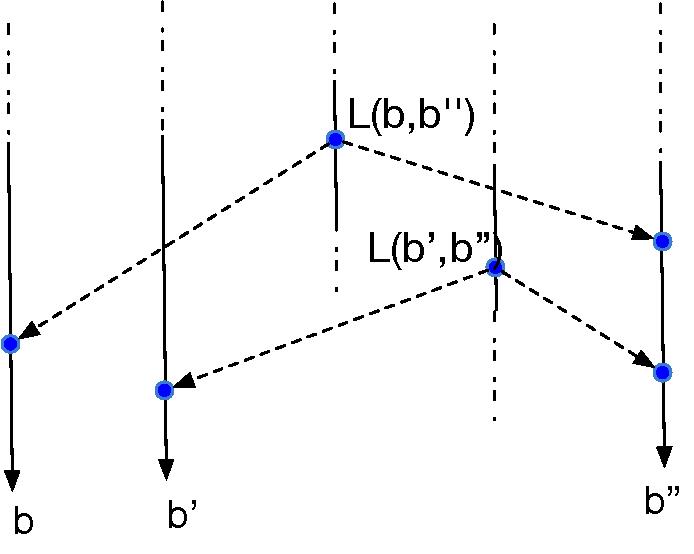
\includegraphics[scale=0.4]{Figures/merge-precondition}
\caption{Explanation for the premise $L(b,b'') \reaches L(b',b'') \disj L(b',b'')
          \reaches L(b,b'')$ on the \rulelabel{Merge} rule.}
\label{fig:merge-precondition}
\end{figure}

\rulelabel{Merge} describes the semantics of merging the head of a
branch $b'$ into $b$ resulting in an new version $v$ on $b$.
Intuitively, \rulelabel{Merge} models the information exchange between
replicas. The two pre-conditions specified using the strict superset
relation ($\supset$) require each of the merging versions, $H(b)$ and
$H(b')$, to include at least one commit not present in their common
ancestor $L(b,b')$. These conditions ensure that the merge is not
trivial (trivial merge is handled by \rulelabel{FastFwd}). The next
pre-condition is key to ensuring the uniqueness of LCAs and the
linearity of merges. It requires that, for every branch $b''$ in the
system, the LCA of $b''$ with merging branches $b$ and $b'$ be
causally related, i.e, $L(b,b'') \reaches L(b',b'') \disj L(b',b'')
\reaches L(b,b'')$. Fig.~\ref{fig:merge-precondition} helps visualize
this condition in the most general case when (\rom{1}). Branches $b$,
$b'$, and $b''$ are distinct, and (\rom{2}). Their LCAs $L(b,b'')$ and
$L(b',b'')$ lie on a distinct pair of branches not equal to $b$, $b'$,
and $b''$. In the figure, once you merge $b'$ into $b$, every version
$v$ that is an ancestor of $L(b',b'')$, i.e., $v \reaches L(b',b'')$,
will be  a common ancestor of $H(b)$ and $H(b'')$. Clearly,
$L(b',b'')$ is the lowest among such common ancestors. But the current
lowest common ancestor of $b$ and $b''$ is $L(b,b'')$. We therefore
end up with two lowest common ancestors -- $L(b',b'')$ and $L(b,b'')$,
\emph{unless} both are ancestrally related. Thus the pre-condition
$L(b,b'') \reaches L(b',b'') \disj L(b',b'') \reaches L(b,b'')$. If
$L(b',b'') \reaches L(b,b'')$, then $L(b,b'')$, the current LCA of $b$
and $b''$, is still the LCA after the merge. On the other hand, if
$L(b,b'') \reaches L(b',b'')$, then $L(b',b'')$ becomes the lowest
common ancestor of $b$ and $b''$ after the merge. Thus $L(b,b'')$
needs to be updated if and only if $L(b,b'') \reaches L(b',b'')$. The
conclusion of the \rulelabel{Merge} captures this update using the set
comprehension notation. It also updates the LCA of the merging
branches $L(b,b')$ to $H(b')$ since the head of $b'$ is merged into
$b$. Updates to the other components of the state (e.g., $C$) follow
the same rationale as previous rules. Two edges are added to $E$ as
the new version $v$ is a descendant of the two merging versions.

Another notable aspect of the \rulelabel{Merge} rule is the invocation
of the \C{merge} function on the values of the  merging versions and
their common ancestor to derive the result of the merge. As explained
above, our development is parameterized on the domain of values for
which a \C{merge} function is defined. No further constraints are
imposed on \C{merge}. We use an uncurried version of \C{merge} to
avoid clutter.

\rulelabel{FastFwd} generalizes merge to the case when the merging
version $H(b')$ is a descendant of the version $H(b)$. In this case
$H'(b)$, the new head of $b$, needs to have the same value and same
set of commits as $H(b')$. Other premises and conclusions are similar
to the \rulelabel{Merge} rule. Note that we don't need a separate rule
for fast forward merge if \C{merge} satisfies the invariant that
$\forall n, n'.~ \C{merge}(n,n,n') \,=\, \C{merge}(n,n',n) \,=\, n$.
Having a separate rule lets us elide this constraint.

\paragraph{Properties} We now formalize the notable properties of the
abstract machine and its executions\footnote{
  The manual proofs of the theorems and their Ivy
  formalization~\cite{ivy} can be found in the supplementary material.
}. 

\begin{lemma}[Uniqueness of LCA]
  \label{lem:lca-uniqueness}
  In every reachable state $\Delta = (G,N,C,H,L)$ of the abstract
  machine, every pair of branches $b_1, b_2 \in dom(H)$ has a unique
  LCA given by $L(b_1,b_2)$.
\end{lemma}

The intuition behind the proof is succinctly captured by
Fig.~\ref{fig:merge-precondition}, which is explained above.

\begin{lemma}[Commit sets grow monotonically]
  \label{lem:commit-monotonicity}
  In every reachable state $\Delta = ((V,E),N,C,H,L)$ of the abstract
  machine: Forall $v_1,v_2 \in V$, if $v_1 \reaches v_2$ then $C(v_1)
  \subseteq C(v_2)$.
\end{lemma}

Lemma~\ref{lem:commit-monotonicity} guarantees that merges never lose
a commit.

\begin{corollary}[Commit sets modulo LCA are disjoint]
  \label{lem:commit-disjointness}
  In every reachable state $\Delta = ((V,E),N,C,H,L)$ of the abstract
  machine: Forall distinct $b_1, b_2 \in dom(H)$, and $v_0, v_1, v_2
  \in V$ s.t.  $v_1 = H(b_1)$ and $v_2 = H(b_2)$ and $v_0 =
  L(b_1,b_2)$, the following is true: $(C(v_2) - C(v_0)) ~\cap~
  (C(v_1) - C(v_0)) = \emptyset$.
\end{corollary}

Corollary~\ref{lem:commit-disjointness} follows from
Lemmas~\ref{lem:lca-uniqueness} and~\ref{lem:commit-monotonicity}.

\begin{theorem}[{\bf Convergence}]
  \label{thm:convergence}
  In every reachable state $\Delta$ = $((V,E),N,C,H,L)$ of the abstract
  machine: Forall distinct $b_1, b_2 \in dom(H)$, and $v_1, v_2 \in V$
  such that $v_1 = H(b_1)$ and $v_2 = H(b_2)$, the following is true:
  $C(v_1) = C(v_2) \Rightarrow N(v_1) = N(v_2)$.
\end{theorem}

Theorem~\ref{thm:convergence} is the key result of this section. It
asserts that any two branches that witnessed the same set of commits
have the same value. Intuitively, this means that any two replicas
that witnessed the same set of user actions arrive at the same final
state \emph{regardless} of the order in which they are witnessed. 

Convergence is vacuously true if the abstract machine never lets any
merges to happen, i.e., if the premises of the \rulelabel{Merge} rule
are too strong to be never true. We prove that this is not the case
with help of the following theorem:

\begin{theorem}[{\bf Progress}]
  \label{thm:progress}
  Every reachable state $\Delta = ((V,E),N,C,H,L)$ of the abstract
  machine is either: 
  \begin{itemize}
    \item A ``quiescent'' state, where: $\forall b_1,b_2 \in
      dom(H).~C(H(b_1)) = C(H(b_2))$, Or
    \item An ``unstuck'' state, where there exist $b_1,b_2 \in dom(H)$
      that satisfy the pre-conditions of \rulelabel{Merge} or
      \rulelabel{FastFwd} rules, i.e., $b_1$ and $b_2$ are mergeable. 
  \end{itemize}
\end{theorem}

Convergence and Progress together ensure the soundness of the \quark
abstract machine.
